\begin{figure}[h]
    \centering
    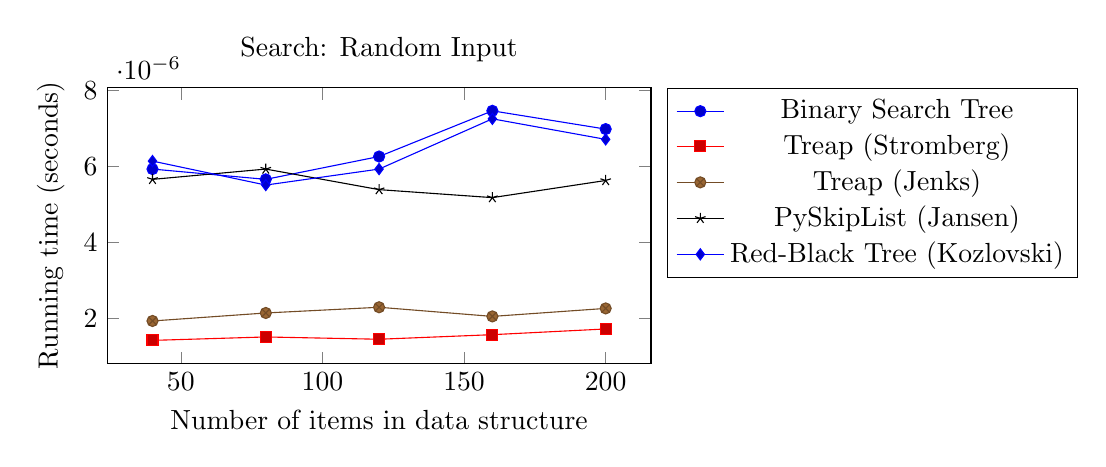
\begin{tikzpicture}
        \begin{axis}[
            xlabel={Number of items in data structure},
            ylabel={Running time (seconds)},
            title={Search: Random Input},
            width=0.7\textwidth,
            height=2in,
            legend pos=outer north east
        ]
		\addplot coordinates {
			(40, 5.933154134007967e-06)
			(80, 5.662096330932842e-06)
			(120, 6.264447004436513e-06)
			(160, 7.46914835144108e-06)
			(200, 6.987267812638698e-06)
		};
		\addplot coordinates {
			(40, 1.4155240827318226e-06)
			(80, 1.5058766837577896e-06)
			(120, 1.445641616407145e-06)
			(160, 1.5661117511084343e-06)
			(200, 1.716699419485046e-06)
		};
		\addplot coordinates {
			(40, 1.927522155209527e-06)
			(80, 2.138344890936783e-06)
			(120, 2.288932559313395e-06)
			(160, 2.0479922899108162e-06)
			(200, 2.2588150256380725e-06)
		};
		\addplot coordinates {
			(40, 5.662096330932842e-06)
			(80, 5.933154134007967e-06)
			(120, 5.391038527854941e-06)
			(160, 5.1802157921304605e-06)
			(200, 5.63197879725752e-06)
		};
		\addplot coordinates {
			(40, 6.143976869737999e-06)
			(80, 5.511508662559006e-06)
			(120, 5.933154134007967e-06)
			(160, 7.258325615716599e-06)
			(200, 6.716210009560797e-06)
		};
        \legend{Binary Search Tree, Treap (Stromberg), Treap (Jenks), PySkipList (Jansen), Red-Black Tree (Kozlovski)}
        \end{axis}
    \end{tikzpicture}
    \caption{Average of 10 operations, benchmarked every 40, starting at 40.}
\end{figure}